    \documentclass[MSc,english]{Container/thesistemplate}
\usepackage[Lenny]{fncychap}
\usepackage[nottoc]{tocbibind}
\usepackage{wrapfig}
\usepackage[font={small,it}, labelfont=bf]{caption}
\usepackage{multicol}
\usepackage{enumitem}

\begin{document}

\author{Federico Vincenzo Mastellone}
\title{Understanding oscillopathies in the Cortico-Basal Ganglia-Thalamocortical loop: an approarch with three heterogeneous populations of Kuramoto oscillators}
\aayear{2021/2022}

\begin{supervisors}
   \supervisor{}{Prof.}{E. Cataldo}
\end{supervisors}

\begin{cosupervisors}
   \cosupervisor{}{Prof.}{A. Mazzoni}
\end{cosupervisors}

\maketitlepage

\tableofcontents

\chapter*{Introduction}
\addcontentsline{toc}{chapter}{Introduction}


\chapter{Background}
\section{The Basal Ganglia Complex}
Among the various complex structures one can find in a mammal's brain the Basal Ganglia \textbf{(BG)} is one of those whose basic anatomy and connectivity hasn't ran into much change in half a billion years \cite{evol} \cite{nelsonkreitzer}.
\\ It is located at the base of the forebrain and it consists of several nuclei; these nuclei form a highly \emph{non linear network} so that each nucleus projects, somehow, to itself and the others. Some of these nuclei also project and receive projections from structures outside the BG --- the \emph{Striatum} and the \emph{Globus Pallidus} are an example, being connected to the \emph{Thalamus} and the \emph{motor Cortex}.
\\ One question rapidly arises: \emph{why had this complex been preserved during evolution? What is its purpose?}
\\ The BG are principally involved in the selection and implementation of purposeful actions in response to external and internal cues. This means that this structure is involved in those tasks in which a facilitation or a suppression of a movement is required. On top of that, it is involved in a series of fundamental non-motor behaviours such as: \emph{emotions}, \emph{language}, \emph{procedural learning} and last but not least \emph{decision making} \cite{simonyan}. It is worth adding that \emph{Dopamine} --- a \emph{neurotransmitter} which is involved in the processing of reward after the completion of a task --- is produced in the BG and plays a crucial role in controlling motor functions and in learning new motor skills.

\subsection{Anatomy}
From a general point of view, the BG complex --- such as any complex in the brain --- consists of some input nuclei, some output nuclei and some internal nuclei whose role is that to process the signals incoming in the input nuclei.
\\ Briefly, this is the list of nuclei composing the Basal Ganglia:

\begin{itemize}
    \item The \emph{Striatum} $\longleftrightarrow$ \textbf{(Str)}, which is formed by 
    \begin{enumerate}
        \item \emph{Putamen}
        \item \emph{Caudate nucleus}
    \end{enumerate}
    
    \item The \emph{Globus Pallidus}, generally divided into
    \begin{enumerate}
        \item the \emph{internal} part $\longleftrightarrow$ \textbf{(GPi)}
        \item the \emph{external} part $\longleftrightarrow$ \textbf{(GPe)}
    \end{enumerate}
    
    \item The \emph{Substantia Nigra}, consisting of
    \begin{enumerate}
        \item its \emph{Pars Compacta} $\longleftrightarrow$ \textbf{(SNc)}
        \item its \emph{Pars Reticulata} $\longleftrightarrow$ \textbf{(SNr)}
    \end{enumerate}
    
    \item The \emph{Subthalamic Nucleus} $\longleftrightarrow$ \textbf{(STN)}
\end{itemize}

\begin{figure}[ht!]
  \centering
    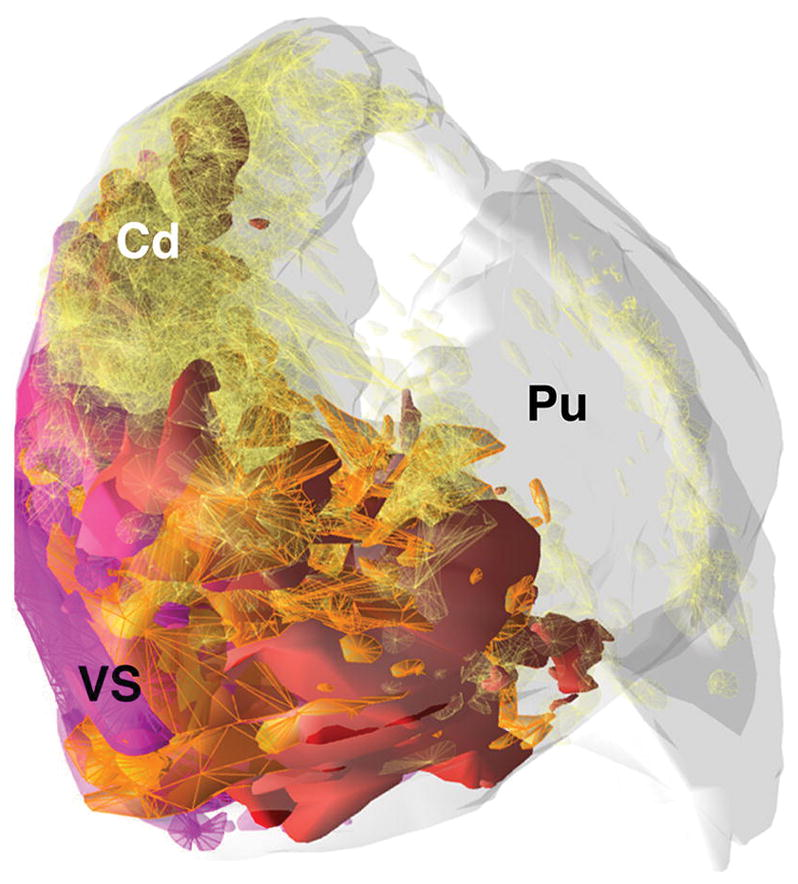
\includegraphics[scale=.8]{Images/striatumrec.jpg}
    \caption{Three dimensional reconstruction of the Striatum including the \emph{Caudate} \textbf{(CD)}, the \emph{Putamen} \textbf{(PD)} and the \emph{Ventral Striatum} \textbf{(VS)}. (Figure adapted from \cite{striatalfigure}).}
    \label{fig:striatum3d}
\end{figure}

\subsection*{Input nuclei}
The \textbf{Striatum}, artistically represented in Figure \ref{fig:striatum3d}, is the major input structure of the Basal Ganglia receiving projection from the Thalamus and pretty much every cortical area. These cortical areas can be grouped into regions each related to a different function: \emph{sensorimotor}, \emph{cognitive} and \emph{affective}; each of these sends excitatory projections to subregions of the Striatum forming distinct channels. There is evidence pointing out that these channels are overlapping and this may serve an integrative function between cognitive, motor and limbic signals deriving from cortical areas. 
\\  Excitatory projections from the Thalamus are topographically organized and overlapping in a similar fashion as the cortico-striatal projections. \cite{nelsonkreitzer}.
\\ In addition to the inputs received from areas outside the Basal Ganglia, the Striatum also collects projections from the SNc and the \emph{Ventral Tegmental Area} \textbf{(VTA)}; these afferent are extremely important since the main neurotransmitter released in the synaptic cleft is \emph{dopamine}. 

\begin{figure}[ht!]
    \centering
    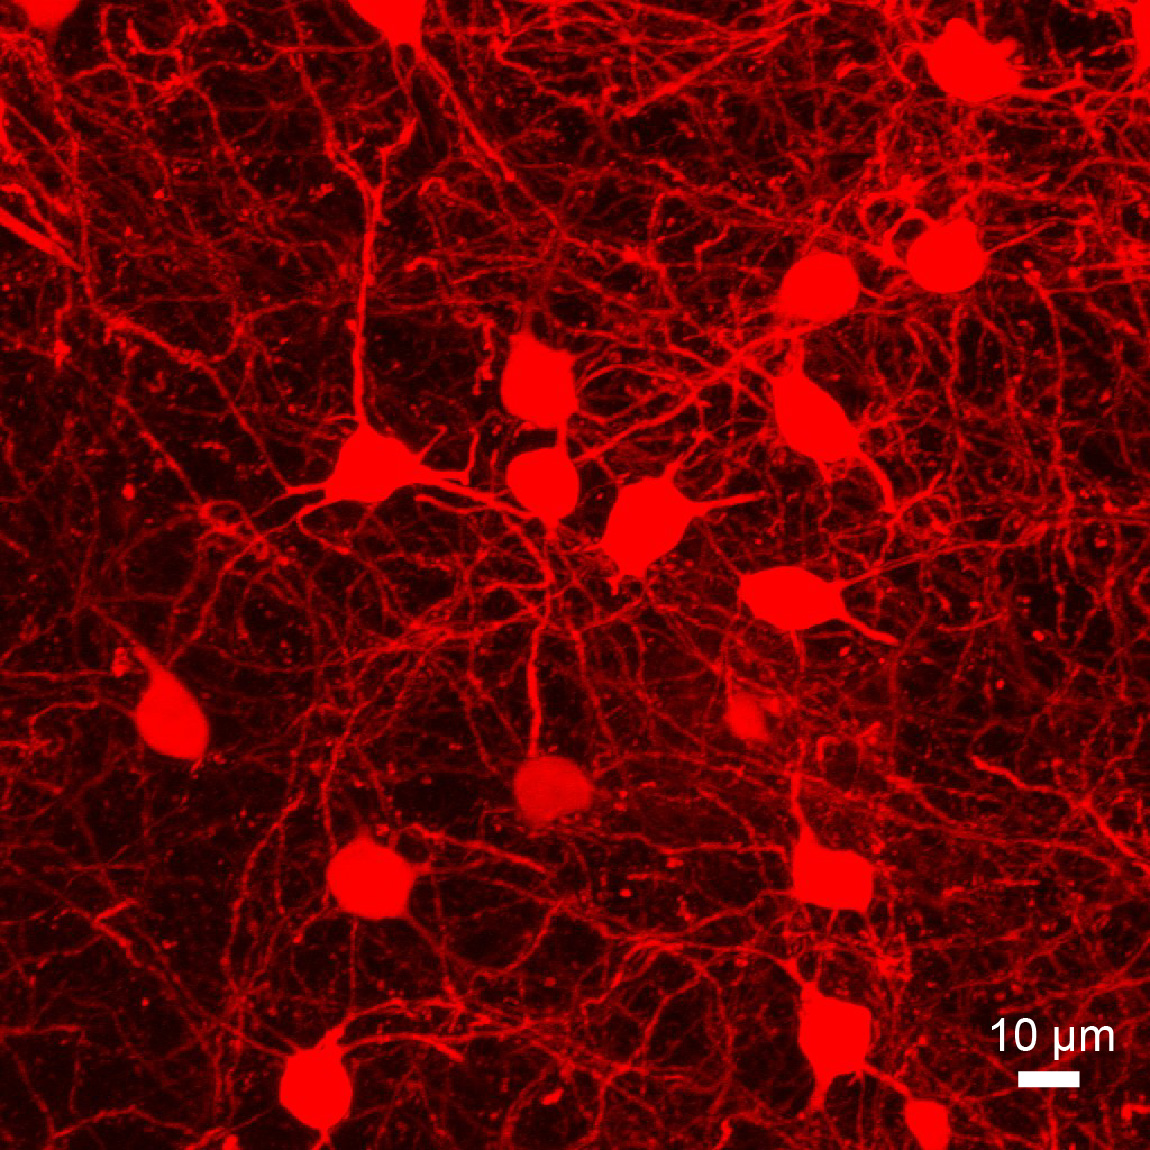
\includegraphics{Images/MediumSpinyNeurons.jpg}
    \caption{Confocal microscopy Z projection of medium spiny neurons (MSNs) in the mouse striatum.}
    \label{fig:msn}
\end{figure}

Among the total number of neurons in this structure, $N_{Str}=(2,791\pm 188)\cdot 10^3$ \cite{oorschot}, 95\% of them are \emph{Medium Spiny Neurons} \textbf{(MSNs)} (Figure \ref{fig:msn}), a type of GABAergic inhibitory neuron, which can be divided in those having the D1-type dopamine receptors and those having the D2-type dopamine receptors; the difference consists in the chemical processes deriving from the \emph{neurotransmitter-receptor} bound. D1 receptors initiates a second messenger-signaling cascade resulting in the depolarization of the post-synaptic MSN, while the same process results in the hyperpolarization of the post-synaptic MSN having the D2 receptor \cite{utterbasso}. Hence, the role of D1 receptors is to enhance cortico-striatal influence and this is in contrast to the reduction mediated by D2 receptors.
\\ Approximately half of the MSNs projects directly to the SNr or the GPi while the remaining half points to the GPe. Dopamine has thus a remarkable influence on the processing of the signals incoming from the Cortex and travelling towards the other BG nuclei.
\\ The other input nucleus in the BG is the \textbf{Subthalamic Nucleus} which, as the name suggests, is positioned just under the Thalamus and it's composed primarily of \emph{glutamatergic neurons}, $N_{STN} = (13.56\pm 1.41)\cdot 10^3$ \cite{oorschot}. As the Striatum the STN receives projections from the \emph{Primary Motor Cortex}, the \emph{Supplementary Motor Cortex} and the \emph{Premotor Cortex} but in a smaller amount. Also, it has afferents coming from the GPe. The STN is the \emph{only} nucleus in the \emph{whole} Basal Ganglia complex to \emph{send excitatory projections}, specifically to the GPi and to the SNr. Some studies' evidences also identify projections from the STN back to the GPe and the Striatum \cite{nelsonkreitzer}.

\subsection*{Intrinsic nuclei}
As suggested in the aforementioned list, the \emph{Globus Pallidus} can be divided into two parts, the interal one and the external one. The \textbf{external part} can be called an \emph{intrinsic nucleus} given that it receives projections from nuclei belonging to the BG, such as the Striatum and the STN, and it sends projections back to almost every BG nucleus \cite{nelsonkreitzer}. It comprises $N_{GPe} = (45.96 \pm 5.12)\cdot 10^3$ GABAergic neurons \cite{oorschot}. Among the intrinsic nuclei in the BG one could also add the \textbf{SNc} and the VTA. These regions contain \emph{dopaminergic neurons} projecting to the Striatum, this means that the main neurotransmitter released is \emph{dopamine} although there's evidence that they can also release \emph{Glutamate} and \emph{GABA} \cite{nelsonkreitzer}. The SNc comprises $N_{SNc} = (7.20 \pm 1.08) \cdot 10^3$ neurons \cite{oorschot}.

\subsection*{Output nuclei}
Some of the Basal Ganglia nuclei send projections to fereign structures, these are called \emph{output nuclei}. The \textbf{SNr} and the \textbf{internal part} of the \emph{Globus Pallidus} fall into this category. The \emph{Pars Reticulata} in the Substantia Nigra comprises $N_{SNr} = (26.32 \pm 1.73) \cdot 10^{3}$ neurons \cite{oorschot} while the \emph{GPi} comprises $N_{GPi} = (3.17 \pm 0.30) \cdot 10^{3}$ neurons, \cite{oorschot} in both cases these neurons are \emph{GABAergic}.
\\ The output nuclei send projections to several \emph{Brainstem} nuclei --- like the \emph{Superior Colliculus} and the \emph{Pedunculopontine Tegmental nucleus} --- which are involved in the regulation of eye movements, in orienting behaviours and in motor and attentional control mechanisms \cite{nelsonkreitzer}. Moreover GPi sends --- but also receives --- projections to the \emph{Thalamus}. The latter is then connected to the \emph{Primary Cortex}. 
\\ As mentioned before, the Primary Cortex's Pyramidal neurons connect to the Striatum; collecting all the informations given so far one can begin to see the formation of an intricate circuit involving the Basal Ganglia nuclei, the Thalamus, the Primary Cortex and some nuclei in the Brainstem.
\\
\\
\\
In Figure \ref{fig:bgnuclei} one can see the Basal Ganglia as a whole artistically represented:

\begin{figure}[ht!]
    \centering
    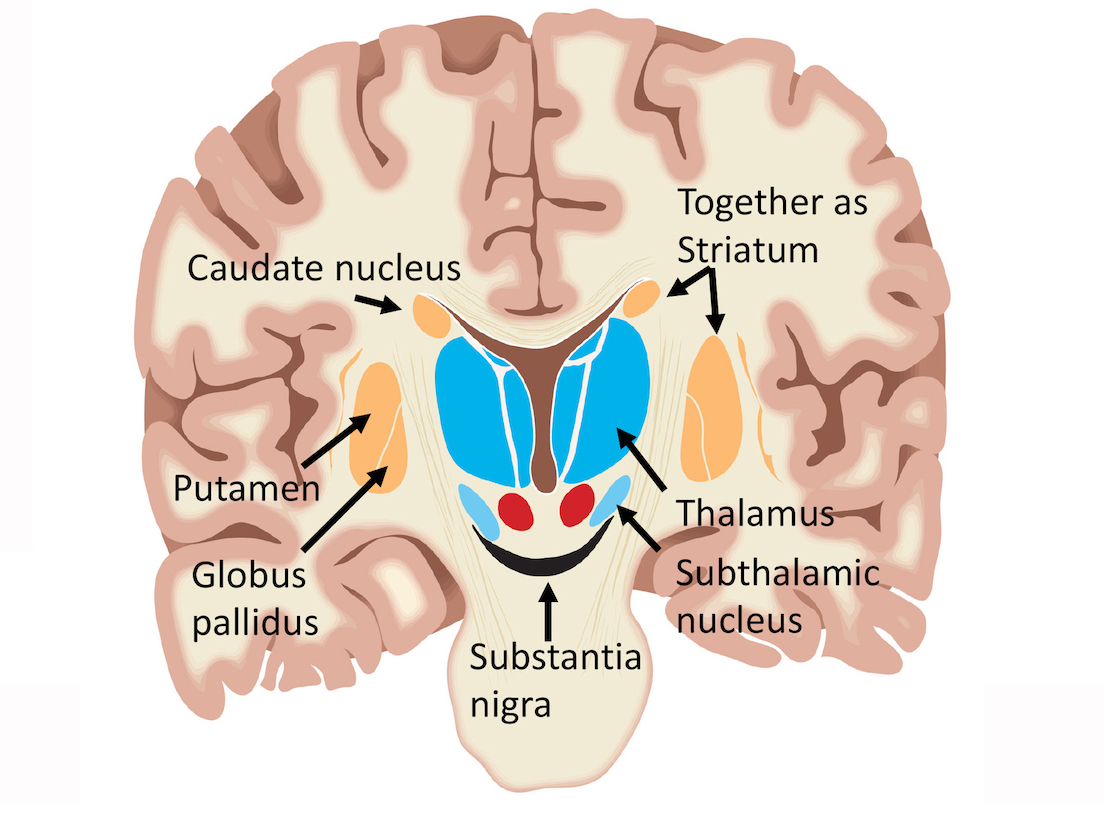
\includegraphics[scale=.3]{Images/bgnuclei.jpg}
    \caption{Artistic representation of the fundamental nuclei in the Basal Ganglia complex. Caudate nucleus and Putamen together form the Striatum. Under the Putamen the Globus Pallidus shows up. In the most internal part of the Basal Ganglia one can see the Subthalamic nucleus and the Substantia Nigra. Although it is not comprehended in the Basal Ganglia nuclei, one can also see in the figure the Thalamus. (Figure adapted from \cite{bgnuclei}).}
    \label{fig:bgnuclei}
\end{figure}

\newpage
\subsection*{A higher degree of complexity}
So far the description of the connectivity in the Basal Ganglia brought out a complex network with a certain --- low, indeed --- degree of complexity. In reality, recent studies showed a much more intricate and complex connectivity among the BG nuclei. 
\\ One of the most important finding is the inclusion of the \emph{Cerebellum} in the Cortico-Basal Ganglia-Thalamocortical network. It has been found that the Cerebellum, specifically the \emph{Dentate nuclei} part of it, is connected to the SNr and the GPi. These connections are intriguing considering the also newly-found Cortico-Pallidal and Cortico-Nigral connections \cite{milardi}.
\\ A detailed figure showing all the recently newly found connections among Basal Ganglia nuclei can be found in \cite{simonyan} and is here showed in Figure \ref{fig:network}:

\begin{figure}[ht!]
    \centering
    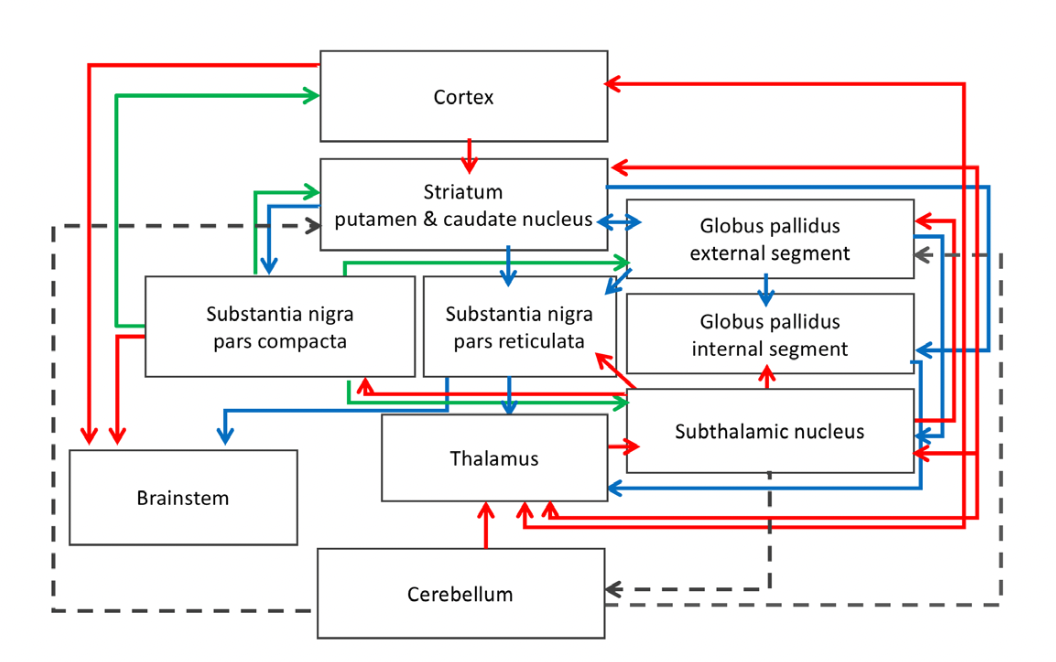
\includegraphics[scale=.75]{Images/network}
    \caption{Schematic representation of Basal Ganglia intrinsic and extrinsic connectivity. Unsurprisingly the network of projections from one nucleus to the others is highly complex. A major challenge arises from such an intricate network and it is represented by the understanding of the physiology in the Cortico-Basal Ganglia-Thalamocortical system.}
    \label{fig:network}
\end{figure}


\newpage
\subsection{Physiology}
Besides the anatomical description of the Cortico-Basal Ganglia-Thalamic complex, another level of characterization could be represented by its physiology, or functionality.
\\Simply put, from a motor perspective, this complex is involved in the selection and implementation of different and possibly competing voluntary movements. Hence, the Basal Ganglia needs to behave so that some of the voluntary movements one wants to do are facilitated and the competing or interfering ones are inhibited \cite{simonyan}.
\\Over the years multiple theories on how the signals coming from the Motor Cortex are processed have been proposed. The classical model --- or GPi rate theory --- presumes the existence of two competing pathways: the \emph{Direct} one and the \emph{Indirect} one (See Figure \ref{fig:gpirate}). Both these pathways link the Striatum to the Output nuclei of the BG in a top-down fashion: 

\begin{itemize}

\item In the direct pathway a subset of neurons in the Striatum sends inhibitory projections directly to the GPi, in turn the GPi sends inhibitory projections to the Thalamus which sends excitatory projections to the Cortex. The resulting behaviour is an increased activity of the Thalamus towards the Cortex.

\item In the indirect pathway a different subset of neurons the Striatum sends inhibitory projections to the GPe which in turn sends its inhibitory projections to the STN. The STN then provides to excite the GPi resulting in an increased inhibition of the Thalamus. The resulting behaviour is a decreased activity of the Thalamus towards the Cortex.

\item The two pathways also differ in the effect that dopaminergic inputs from the SNc have on them. This input is inhibitory on the subset of Striatum's neurons involved in the Indirect pathway while it's excitatory on the subset involved in the Direct pathway \cite{montgomery}.

\end{itemize}

It is quite clear that these two pathways seems to effectively be competing and comprising of all the possible behaviours of the BG. 
\\The evidence, though, contradicts the previous statement: a few studies suggest that the STN is directly reached by Cortical projections, in turn it ``classically'' sends excitatory projections to the GPi. This newly discovered pathway has been labeled as \emph{Hyperdirect} \cite{simonyan}.
\\Another important revision of the classical model is related to the interaction between the two principal pathways. In principle it seemed that the two pathways were \emph{parallel} and \emph{segregated} but different studies demonstrated that there is, indeed, a cross-talk between them. In fact, \emph{bridging collaterals} have been found between the pathways whose density seems to be directly proportional to an increased pallidal inhibition \cite{simonyan}.

\begin{figure}[ht!]
    \centering
    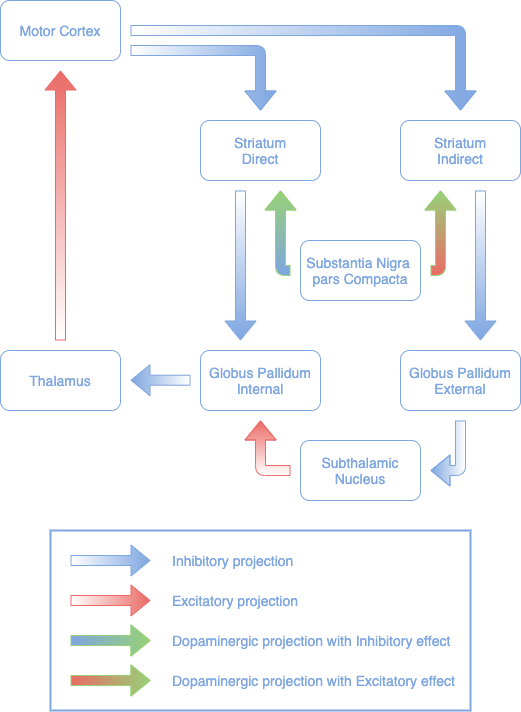
\includegraphics[scale=.4]{Images/gpiratetheory}
    \caption{Graphic representation of the GPi rate model. As it is reported in the legend, blue arrows represent inhibitory projections, red arrows represents excitatory projections, green arrows represents dopaminergic projections sent by the SNc having two possible post-synaptic effects on the Striatum. Starting from the Striatum, two different pathways are highlighted, the shorter one is the Direct one, linking the Striatum directly to the GPi, the longer one is, hence, the Indirect one, reaching the GPi only after meeting the GPe and, subsequently, the STN.}
    \label{fig:gpirate}
\end{figure}

\newpage
A different approach to the physiology of the Cortico-Basal Ganglia-Thalamocortical complex can be found in \cite{montgomery}. In the previously showed model the system is organized in a \emph{sequential} and \emph{hierarchical} way, in contrast, in the \emph{Systems Oscillators theory} the system is viewed as a collection of multiple nested, loosely coupled, dynamic, non-linear, reentrant and polysynaptic oscillators \cite{montgomery}. This model solves a few issues that arise when one tries to explain data gathered from patients with \emph{Parkinson Desease} using the GPi Rate model, these will be addressed in the next section.

\begin{figure}[ht!]
    \centering
    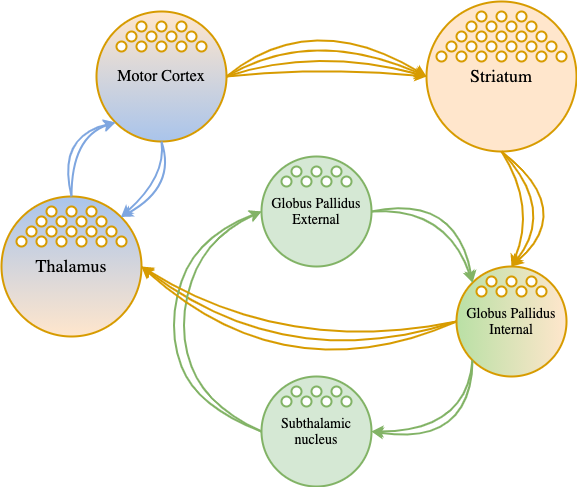
\includegraphics[scale=.5]{Images/systemsoscillatorstheory2}
    \caption{Graphic representation of the Systems Oscillators model. As is it possible to notice, three oscillators can be found in this model, the thalamocortical one being the main one. Each node of each oscillator is, in fact, a nucleus of the Cortico-Basal Ganglia-Thalamocortical system which is represented in the figure having an oval shape. Anatomically speaking, each nucleus comprises a different number of neurons, in the figure this is represented by a higher number of overlapping ovals. Each node projects to the next one regardless of the type of projection.}
    \label{fig:sysosc}
\end{figure}

In this model oscillators comprise different nuclei in the Basal Ganglia complex, the Thalamus and the motor part of the Cortex as nodes in each oscillator. Nodes might have a different number of neurons, reflecting the anatomical differences of each nucleus. Each neuron in a node --- or nucleus --- might not produce a spike within an oscillator's cycle but there is, in each node, a sufficient number of neurons in order to let the oscillations keep going. Quoting Montgomery himself \cite{montgomery}: 
\\
\\\emph{``This probabilistic rate divider function of the neurons, in addition to other non-linearities, prevents saturation or collapse of the oscillators, issues that lead to rejection of the notion of reentrant oscillators [...] in the 1930s.''}
\\
\\The projection from a node to another in the same oscillator might be \emph{inhibitory} or \emph{excitatory}; one could think that an inhibitory projection actually lessen the capacity of the oscillation to propagate through subsequent nodes, this is a misleading thought, at least for two reasons: the Basal Ganglia complex is, indeed, an inhibitory driven complex, the second reason is related to the possibility of a \emph{Post-Inhibitory Rebound Spike} of the post-synaptic neuron after a high degree of hyperpolarization of its membrane voltage. These two reason should convince the reader that there is, indeed, a way to let the signal propagate in the oscillator.
\\This model correctly predicts some of the evidences in the Basal Ganglia complex: the coherence between \emph{Local Field Potentials} (LFP) registered in subsequent nodes of the loops, the naturally lesser frequency in the registered activity of a single neuron if compared to the frequencies of the oscillations in the LFP, the correlation Local Field Potentials and the spiking of a neuron in the same region and, finally, that a \emph{lesion} in \emph{any} point of the oscillator --- hence in any of the nuclei involved in a specific loop --- causes the same symptoms.
\\In the System Oscillators model the main loop is the one involving the \emph{Thalamus} and the \emph{motor Cortex}, hence the other loops have the role of modulators of the amplitude and the frequency of oscillation of the main loop. This creates the perfect balance of muscle forces for an optimal movement.
\\In the case of \emph{dopamine depletion}, as stated in \cite{montgomery}, an increase in the coupling of the oscillators in the BG-Th-Ctx system could happen, this leading to a reduction of the \emph{complexity} of neuronal activities necessary for a normal behaviour.

\newpage
\section{Momevent disorders: a link with the Basal Ganglia}
There's a fairly abundant list of pathologies related to movement, or \emph{movement disorders}.  Below a brief list containing the most studied ones:

\begin{itemize}
\begin{multicols}{2}
	\item Parkinson's disease
	\item Dystonia
	\item Chorea
	\item Huntington's disease
	\item Essential tremor
	\item Tourette's syndrome
\end{multicols}
\end{itemize}

These movement disorders are characterized by the difficulty of starting or completing a specific movement. These difficulties can be categorized in two groups: \emph{hypokinesias} and \emph{hyperkinesias}. \emph{Hypo} and \emph{hyper} are ancient greek words meaning, respectively,  \emph{under, less} and \emph{above, exceeding} while \emph{kinesia}, still coming from greek, means \emph{movement}. Hence these pathologies are characterized by symptoms related to the incapability to perform a specific movement and/or the incapability to control involuntary, fast-paced and sudden, movements.
Some of these symptoms are listed in Table \ref{tab:hypok} and Table \ref{tab:hyperk}, below.

\begin{table}[ht!]
\centering

\begin{tabular}{ll}
\multicolumn{2}{c}{I. Hypokinesias} \\
\hline
A. Akinesia/Bradykinesia & C. Rigidity \\
B. Catatonia &  D. Stiff muscles \\
\hline
\end{tabular}

\caption{A brief list of hypokinetic symptoms in movement disorders. These symptoms limit and drastically slow down the movements that a person tries to do.}
\label{tab:hypok}

\vspace*{.5 cm}

\begin{tabular}{ll}
\multicolumn{2}{c}{II. Hyperkinesias} \\
\hline
A. Ataxia/Asynergia/Dysmetria & C. Dystonia \\
B. Hyperekplexia & D. Myoclonus \\
E. Tics & F. Tremors \\
\hline
\end{tabular}

\caption{A brief list of hyperkinetic symptoms in movement disorders. \\ Tables adapted from \cite{fahn}}
\label{tab:hyperk}
\end{table}

Some of the aforementioned pathologies include hypokinetic and hyperkinetic symptoms; Parkinsonism, as an example, is characterized by \emph{bradykinesia}, a hypokinetic symptom, and \emph{tremors}, a hyperkinetic symptom. Other pathologies are strictly characterized by symptoms related to one of the two categories; Tourette's syndrome, for example, is mainly characterized by involuntary \emph{tics} which falls, as a symptom, in the hyperkinetic category.\\
These diseases haven't always been called \emph{movement disorders} as they were initially called \emph{extrapyramidal disorders}; the reason beyond this name is related to the evidence that these disorders stemmed from pathology in the deep nuclei within the cerebral hemispheres, \emph{also known as Basal Ganglia}. 
\\Later on their name was changed to movement disorders being that nuclei in the Basal Ganglia are, indeed, intimately connected to the pyramidal tract system; also, some extra-pyramidal pathways descending through the spinal cord  actually exist and they're not involved in movement disorders \cite{fahn}.\\
Recently it has been showed that such movement disorders are associated with an abnormal synchronization of the Cortico-Basal Ganglia-Thalamocortical network; different pathologies are related to different synchronization frequencies \cite{vissani}. This could lead to the interpretation of such pathologies as \emph{oscillopathies}.

\subsection{Pathophysiology of Parkinson's Desease}
In this brief section the attention is going to be drawn to Parkinson's disease -- \emph{PD}. Subjects affected by Parkinsonism show an abnormal synchronization in the Local Field Potential retrieved from the Globus Pallidus and the Subthalamic Nucleus. This exceeding synchronization happens to exist in the range of frequencies going from 13 to 30 Hz, the so called beta frequency range \cite{vissani}.

\newpage
\section{Oscillapathies in the brain}

\newpage
\section{Deep Brain Stimulation: an empirical treatment}
%\ DBS come oscillatore Montgomery
\subsection{Open Loop}
\subsection{Closed Loop}

\newpage
\section{Oscillators in Physics}
\subsection{The Kuramoto Model}
\subsection{An extension: the Kuramoto-Sakaguchi model}

\newpage
\chapter{Methods and materials}


\bibliographystyle{unsrt}
\bibliography{biblio}
\end{document}